
%\documentclass[mathserif]{beamer}
\documentclass[handout]{beamer}
%\usetheme{Goettingen}
\usetheme{Warsaw}
%\usetheme{Singapore}



%\usetheme{Frankfurt}
%\usetheme{Copenhagen}
%\usetheme{Szeged}
%\usetheme{Montpellier}
%\usetheme{CambridgeUS}
%\usecolortheme{}
%\setbeamercovered{transparent}
\usepackage[english, activeacute]{babel}
\usepackage[utf8]{inputenc}
\usepackage{amsmath, amssymb}
\usepackage{dsfont}
\usepackage{graphics}
\usepackage{cases}
\usepackage{graphicx}
\usepackage{pgf}
\usepackage{epsfig}
\usepackage{amssymb}
\usepackage{multirow}	
\usepackage{amstext}
\usepackage[ruled,vlined,lined]{algorithm2e}
\usepackage{amsmath}
\usepackage{epic}
\usepackage{epsfig}
\usepackage{fontenc}
\usepackage{framed,color}
\usepackage{palatino, url, multicol}
%\algsetup{indent=2em}
\newcommand{\factorial}{\ensuremath{\mbox{\sc Factorial}}}
\newcommand{\BIGOP}[1]{\mathop{\mathchoice%
{\raise-0.22em\hbox{\huge $#1$}}%
{\raise-0.05em\hbox{\Large $#1$}}{\hbox{\large $#1$}}{#1}}}
\newcommand{\bigtimes}{\BIGOP{\times}}
\vspace{-0.5cm}
\title{Sentiment and Emotion Analysis in Social Media}
\vspace{-0.5cm}
\author[Felipe Bravo Márquez]{\footnotesize
%\author{\footnotesize  
 \textcolor[rgb]{0.00,0.00,1.00}{Felipe Bravo-Marquez}} 
  
 
%\vspace{-0.3cm}
\institute{Department of Computer Science, University of Chile \\ Millenium Institute Foundational Research on Data }

\titlegraphic{
\includegraphics[scale=0.1]{pics/logodcc.png} 
\includegraphics[scale=0.6]{pics/imfdlogo.png}}



\date{\today}

\begin{document}
\begin{frame}
\titlepage


\end{frame}


\section{Introduction}





%\begin{frame}{Social Media}
%\begin{scriptsize}
%\begin{itemize}
% \item Social media plattforms are increasingly being adopted by people in order to access and publish information.  
% \item \textbf{Twitter}: Massively used Microblogging platform where users post messages limited to 280 characters referred to as \textbf{tweets}. 
% \item  Tweets can be used to convey  emotions,  opinions, and  stance.
%%
%\begin{figure}[htbp]
%\begin{center}
%\scalebox{0.7}{
%\begin{tabular}{cc}
%
\includegraphics[scale=0.2]{pics/twitter.png} & 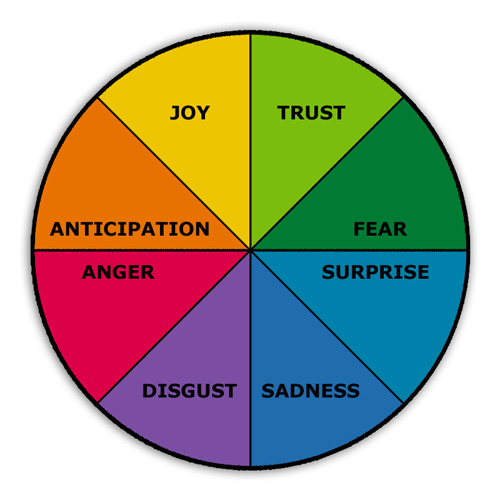
\includegraphics[scale=0.2]{pics/wheel_th.jpg} \\
%\end{tabular}}
%\end{center}
%\end{figure}

%\end{scriptsize}
%\end{frame}



\begin{frame}{Sentiment Analysis and Social Media}
\begin{scriptsize}
\begin{itemize}
 \item Opinions are provided \textbf{freely and voluntarily} by the users in social media. 
 \item Analysing the sentiment underlying these opinions has important applications in product \textbf{marketing} and \textbf{politics}.
 
  \item Warning 1: Twitter and Facebook are not representative of the general population.
  
  \item Warning 2: Mechanisms provided by these plattforms to access posts from public accounts is limited.
 
   \begin{figure}[h]
        	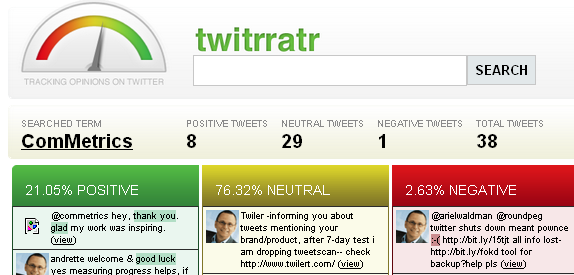
\includegraphics[scale = 0.5]{pics/tweetOpinions.png}
        \end{figure}
\end{itemize}
\end{scriptsize}




\end{frame}


\begin{frame}{Opinion Mining or Sentiment Analysis}
\begin{scriptsize}\begin{itemize}
 \item Application of \textbf{NLP} and \textbf{machine learning} techniques to identify and extract subjective information from textual datasets.
\end{itemize}

\begin{block}{Main Problem: Message-level Polarity Classification (MPC)}
  \begin{enumerate}
   \item Automatically classify a sentence to classes \textcolor[rgb]{0.00,0.00,1.00}{\textbf{positive}}, \textcolor[rgb]{1.00,0.00,0.00}{\textbf{negative}}, or {\textbf{neutral}}. 
   
     \begin{figure}[h]
        	
\includegraphics[scale = 0.15]{pics/sent.png}
        \end{figure}
   
   \item State-of-the-art solutions use \textbf{supervised} machine learning models trained from \textbf{manually} annotated examples \cite{Mohammad2013}.
  \end{enumerate} 
\end{block}

\end{scriptsize}

\end{frame}


\begin{frame}{Sentiment Classification via Supervised Learning}

\begin{figure}[h]
        	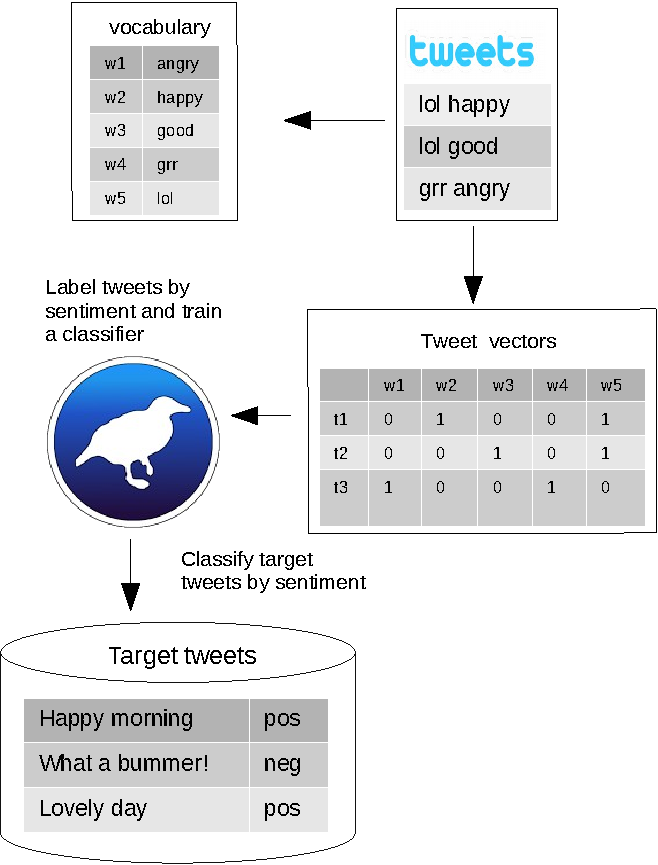
\includegraphics[scale = 0.4]{pics/bagOfwordsClassification.pdf}
        \end{figure}

\end{frame}




%\begin{frame}{Supervised Learning: Support Vector Machines (SVMs)}
%\begin{scriptsize}
%
%\begin{itemize}
%\item Idea: Find a hyperplane that separates the classes with the maximum margin (largest separation). 
%
%     \begin{figure}[h]
%        	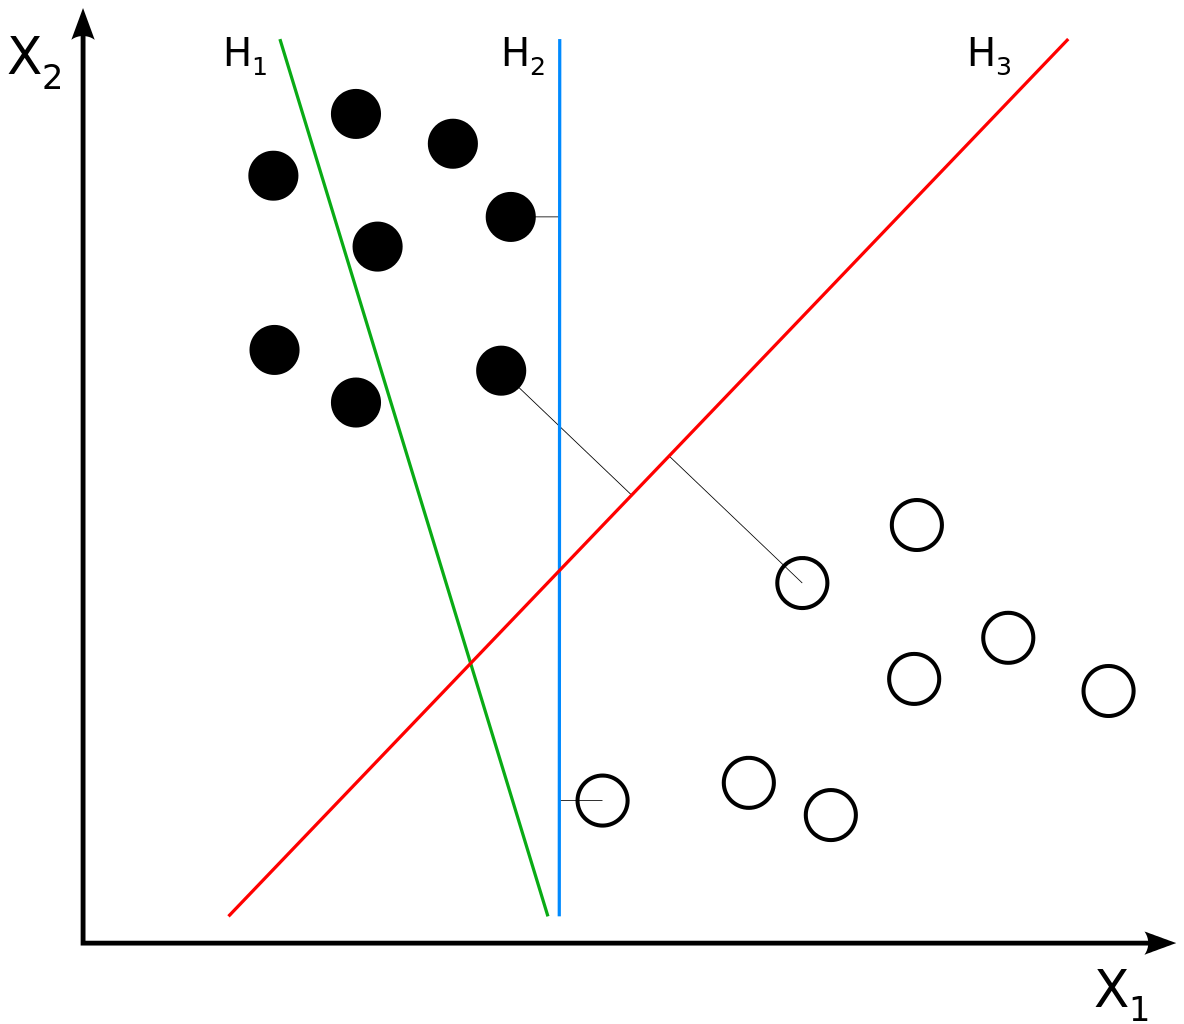
\includegraphics[scale = 0.1]{pics/SVM.png}
%        \end{figure}
%
%\item   
%$H_3$ separates the classes with the maximum margin. 
%
%\end{itemize}
%
%\footnotemark{Image source: Wikipedia}       
%   
%\end{scriptsize}
%
%\end{frame}




%\begin{frame}{Challenges}
%
%Language is complex: negation, compositionality, sarcasm.
%
%
 % 
 % \begin{block}{Examples of complex sentences}
%\begin{enumerate}
%   \item Positive: It's not life-affirming—it’s vulgar and mean, but I liked it.
%\item Negative: It's a disappointing that it only manages to be decent instead of dead brilliant.
%\end{enumerate}
%\end{block}
%  
%
%
%\end{frame}




\begin{frame}{Challenges}
\begin{scriptsize}

\begin{itemize}  
\item \textbf{Label sparsity (LS)}: manual annotation is \textbf{labour-intensive} and \textbf{time-consuming}. 
\item \textbf{Concept drift}: the sentiment pattern can vary from one collection to another (domain-drift, temporal-drift).
 
\item A classifier trained from data annotated for one domain will \textbf{not necessarily} work on another one! 
\item Trained models can become outdated over time.
\end{itemize} 
  
  
\begin{block}{Examples of domain-Drift}
\begin{enumerate}
\item  For me the queue was pretty \textcolor[rgb]{0.00,0.00,1.00}{\textbf{small}} and it was only a 20 minute wait I think but was so worth it!!! :D @raynwise
\item Odd spatiality in Stuttgart. Hotel room is so  \textcolor[rgb]{1.00,0.00,0.00}{\textbf{small}} I can barely turn around but surroundings are inhumanly vast \& long under construction.
\end{enumerate}
\end{block}


\end{scriptsize}

\end{frame}



%\begin{frame}{Approaches to overcome label sparsity}
%\begin{scriptsize}
%\begin{block}{Distant Supervision}
%  \begin{itemize}
%   \item Automatically \textbf{label} unlabelled data (\textbf{Twitter API}) using a heuristic method.
%   \item \textbf{Emoticon-Annotation Approach (EAA)}: tweets with positive \textcolor[rgb]{0.00,0.00,1.00}{\textbf{:)}} or negative \textcolor[rgb]{1.00,0.00,0.00}{\textbf{:(}} emoticons are labelled according to the polarity indicated by the emoticon~\cite{Read2005}.
%  \item The emoticon is \textbf{removed} from the content.
%  \item The same approach has been extended using hashtags \#anger, and emojis.
%\item \textbf{Drawback}: emoticons can induce noisy and incomplete information. Moreover they are not necessarily used in all domains (e.g., politics). 
%\end{itemize} 
%\end{block}
%\end{scriptsize}

%\end{frame}



\begin{frame}{Data Annotation}
\begin{scriptsize}
\begin{block}{Crowdsourcing}
  \begin{itemize}
\item Rely on services like \textbf{Amazon Mechanical Turk} or \textbf{Figure Eight} to ask the \textbf{crowds} to label a sample of the data.


\item Studies show that crowdsourced annotations can be competitive to expert annotations \cite{snow-etal-2008-cheap}.

\item Achieving good annotation quality is challenging: how many annotators per sentence? how much to pay? how to consodolite disagreements? 

\item It is hard to ensure that the annotated sample will cover all the complexities of language usage. 
   \end{itemize} 
 
\end{block}
\end{scriptsize}

     \begin{figure}[h]
        	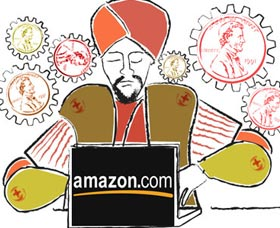
\includegraphics[scale = 0.3]{pics/amt.jpg}
        \end{figure}

\end{frame}


\begin{frame}{Roadmap}
\begin{scriptsize}
\begin{itemize}
\item In the rest of this talk we will overview two dimensions of sentiment analysis.
\item First: sentiment analysis is not a single well-defined problem. We will introduce many popular sentiment analysis \textbf{tasks}.

\item Second: we will overview various techniques used to solve those tasks (e.g, \textbf{feature-based} machine learning, \textbf{deep learning}).

\end{itemize} 

\end{scriptsize}

\end{frame}

\section{Tasks}



\begin{frame}{Fine-grained Sentiment Analysis}

Calculate fine-grained sentiment labels for phrases in the parse trees of a sentences \cite{socher2013recursive}.

    \begin{figure}[h]
        	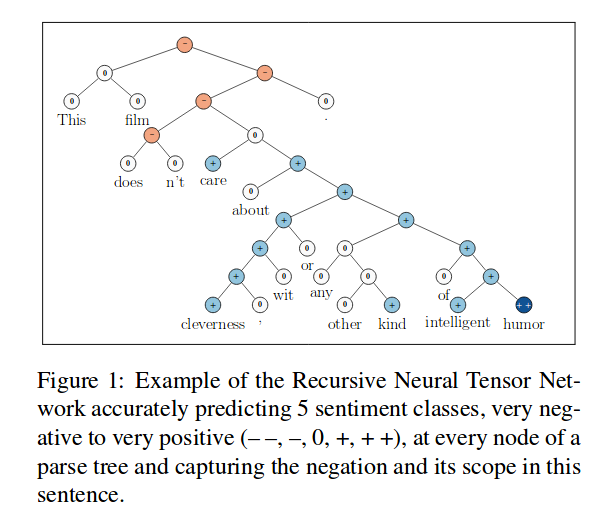
\includegraphics[scale = 0.3]{pics/recTensor1.png}
        \end{figure}   
 



\end{frame}


\begin{frame}{Aspect-based Opinion Mining}

Extract fine-grained information with respect to entities mentioned in user comments \cite{saeidi-etal-2016-sentihood}.

    \begin{figure}[h]
        	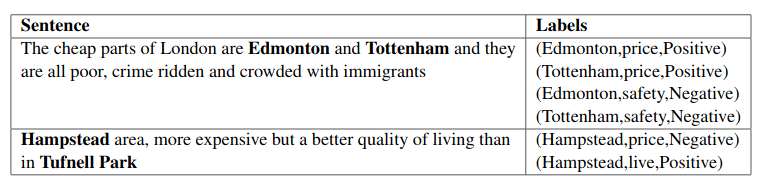
\includegraphics[scale = 0.4]{pics/sentihood.png}
        	
        \caption{Sample sentences taken from the Sentihood dataset.}
        \end{figure} 
 



\end{frame}



\begin{frame}{Stance Detection}
\begin{scriptsize}

 Detect if the author of a tweet is in favor, against or neutral regarding a given target (e.g., Donald Trump). 

     \begin{figure}[h]
        	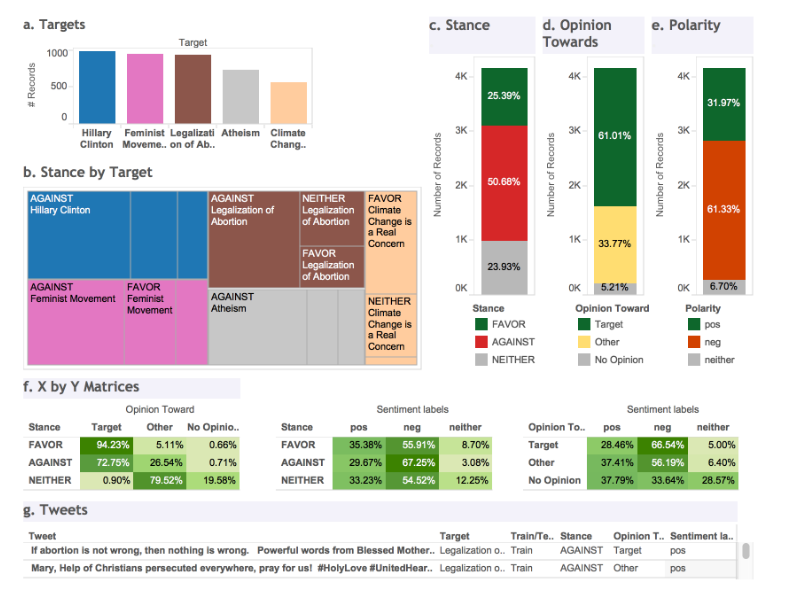
\includegraphics[scale = 0.3]{pics/stance.png}
        \end{figure} 
 
 
\end{scriptsize}

\end{frame}



\begin{frame}{Emotion Intensity Detection}
\begin{scriptsize}
\begin{scriptsize}
\begin{itemize}
\item Given a tweet and an emotion X (anger, fear, sadness, joy) , determine the intensity or degree of emotion X felt by the speaker -- a real-valued score between 0 and 1.
%\item Data was annotated using Best-worst-scaling.
\end{itemize} 

\end{scriptsize}



     \begin{figure}[h]
        	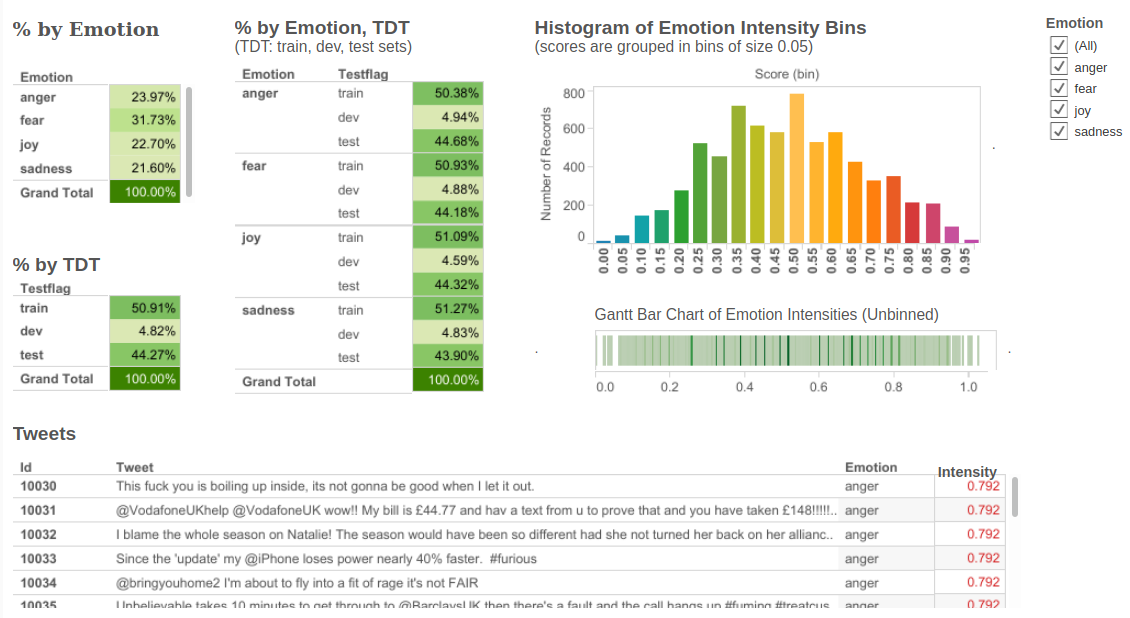
\includegraphics[scale = 0.25]{pics/emoint.png}
        \end{figure} 
 
 
\end{scriptsize}

\end{frame}


%\begin{frame}{Other Tasks}
%
%\begin{itemize}
%
%   \item Hate Speech Detection.
%   \item Irony/Sarcasm Detection: detecting sarcasm in tweets.
%   \item Emotions classification: classify tweets according to multiple emotions (e.g., anger, fear, sadness, joy)
%   \item Lexicon Induction: classification of words into sentiment and/or emotions. 
%
%\item Many of these probems have been evaluated in \textbf{SemEval} tasks.
%
%\end{itemize}
%
%\end{frame}


\section{Models}

\begin{frame}{Rule-based systems}
\begin{scriptsize}
\begin{itemize}
 \item There are various commercial and free rule-based sentiment analysis systems: SentiStrength, Vader, LIWC \footnote{\url{http://liwc.wpengine.com}}.
 
      \begin{figure}[h]
        	
\includegraphics[scale = 0.25]{pics/liwc.png}
        	
\includegraphics[scale = 0.25]{pics/sentistrength.png}
        \end{figure} 
 
 
 \item These techniques use \textbf{opinion or emotion lexicons} together with aggregation rules.
 
 \item These rules deal with sentiment patterns such as negation and intensifiers (e.g., I really don't like onions). 
  \item They are not as strong as machine-learning based systems.
  
  \item However, rule-based systems have the advantage of being easier to interpret and manipulate. 
\end{itemize}
\end{scriptsize}
 
 

\end{frame}






\begin{frame}{Feature-based Systems}
\begin{scriptsize}
\begin{itemize}
\item In 2013, The Semantic Evaluation (SemEval) workshop organised the
``Sentiment Analysis in Twitter
task'' \cite{Semeval2013}.
 \item The tasks involved the automatic classification of tweets into positive, negative and neutral classes.
\item  The organisers released training and testing datasets
for both tasks.
\cite{Semeval2013}

\item The team that achieved the highest performance in both
tasks among 44 teams was the \emph{NRC-Canada} team
\cite{Mohammad2013}.  
\item The team proposed a supervised approach using a linear SVM
classifier with the following hand-crafted features for representing tweets.

\end{itemize}
\end{scriptsize}
\end{frame}

%Tradi7onal: Curated sentiment dictionaries combined with either bag-of-words representa7ons (ignoring word order) or hand-designed nega7on features (aint gonna capture everything) 

% http://cs224d.stanford.edu/lectures/CS224d-Lecture1.pdf

\begin{frame}{Feature-based Systems}
\begin{scriptsize}
\begin{enumerate}
\item  Word $n$-grams.
\item  Character $n$-grams. 
\item Part-of-speech tags.
\item Word clusters trained with the Brown clustering method~\cite{brown1992class}.
\item The number of elongated words (words with one character repeated more than two times).
\item The number of words with all characters in uppercase.
\item The presence of positive or negative emoticons.
\item The number of individual negations.
\item The number of contiguous sequences of dots, question marks and exclamation marks.
\item Features derived from polarity lexicons~\cite{Mohammad2013}. 
\end{enumerate}
\end{scriptsize} 
\end{frame}




\begin{frame}{Feature Engineering and Deep Learning}
\begin{scriptsize}
\begin{itemize}
%\item Up until 2014 most state-of-the-art sentiment analysis systems were based on feature engineering + shallow machine learning models such as linear SVMs.
\item Designing the features of a winning NLP system requires a lot of domain-specific knowledge.
\item The NRC system was built before deep learning became popular in NLP.
\item Deep Learning systems on the other hand rely on neural networks to automatically learn good representations.
\end{itemize}
\end{scriptsize}


      \begin{figure}[h]
        	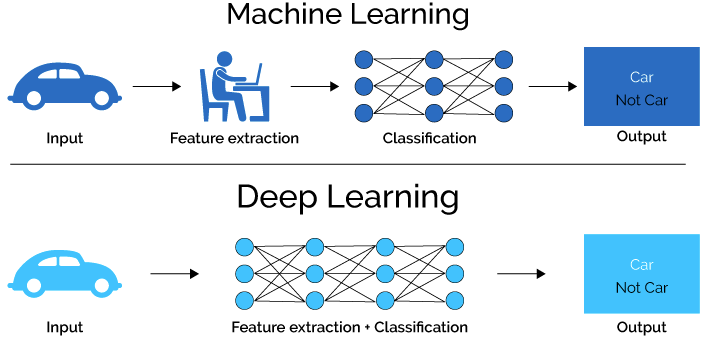
\includegraphics[scale = 0.25]{pics/MLvsDL.png}
        \end{figure} 




\end{frame}


\begin{frame}{Feature Engineering and Deep Learning}
\begin{scriptsize}
\begin{itemize}
\item Deep Learning yields state-of-the-art results in most NLP tasks. 
\item Large amounts of training data and faster multicore GPU machines are key in the success of deep learning. 
\item \textbf{Neural networks} and \textbf{word embeddings} play a key role in modern  sentiment analysis models.
\end{itemize}
\end{scriptsize}
\end{frame}




%\begin{frame}{Word Embeddings}
%\begin{scriptsize}
%\begin{itemize}
%\item  Word \textbf{embeddings} are low-dimensional continuous dense word vectors trained from document corpora using \textbf{neural networks}.
%
%\item Distance between vectors can be equated to distance between words according to the distributional hypothesis. 
%
%\end{itemize}
%\end{scriptsize}
%
% \begin{figure}[h]
%    	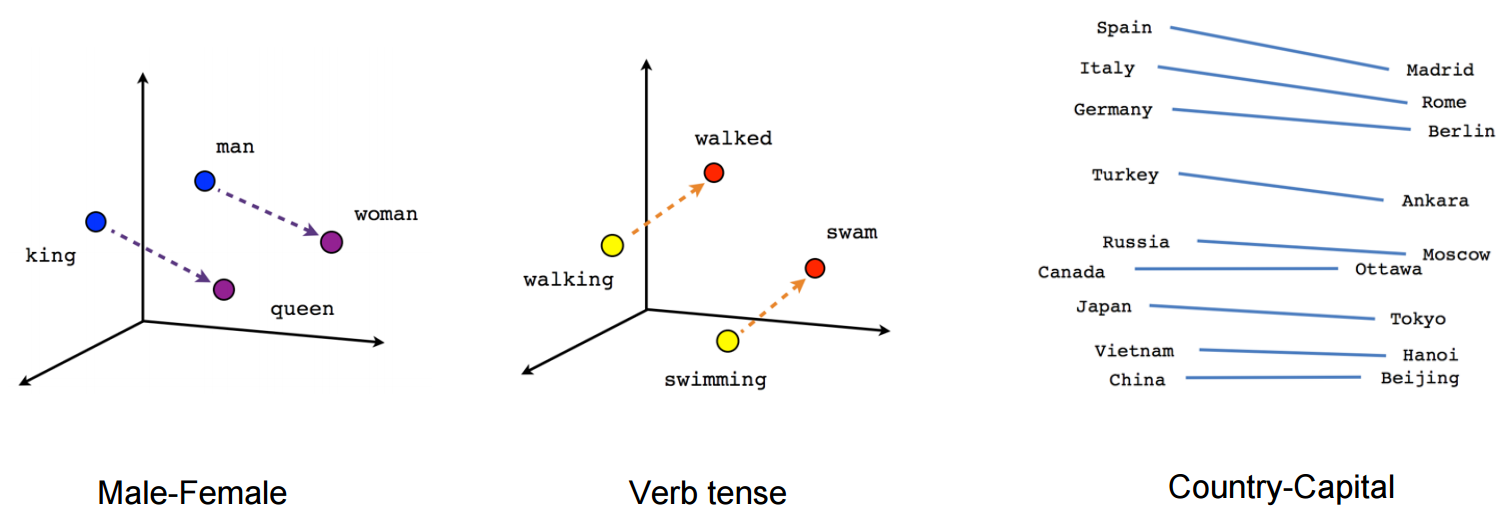
\includegraphics[scale = 0.18]{pics/linear-relationships.png}
%    \end{figure}
%
%
%\end{frame}




%\begin{frame}{Twitter Sentiment Classification with a CNN}
%\begin{scriptsize}
%\begin{itemize}
%\item  The weights of the neural network are pre-trained using emoticon-annotated data, and then trained with the hand-annotated tweets from the SemEval competition.
%\end{itemize}
%  \begin{figure}[h]
%        	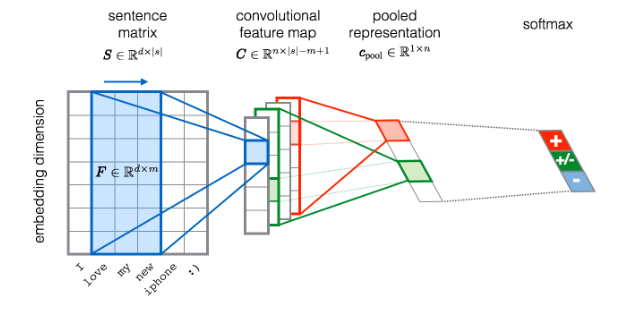
\includegraphics[scale = 0.45]{pics/cnn-twitter.png}
%        \end{figure}
%\end{scriptsize}
%\end{frame}





\begin{frame}{DeepEmoji}
  \begin{figure}[h]
        	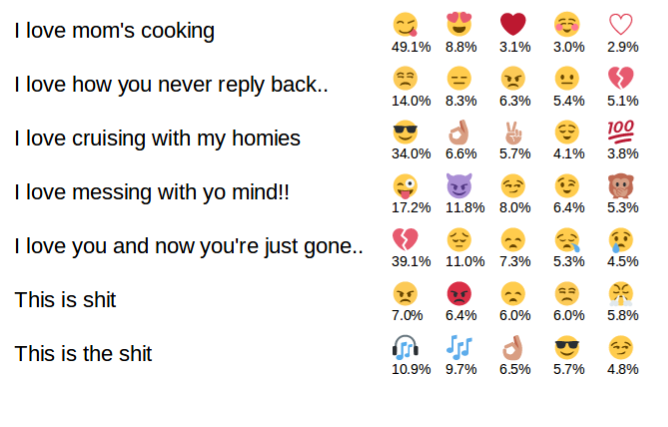
\includegraphics[scale = 0.45]{pics/deepEmoji1.png}
        \end{figure}    
        
\end{frame}






\begin{frame}{Final Comments}
\begin{scriptsize}
\begin{itemize}
%\item Most recent approaches use contextualized pre-trained models such as BERT. 
\item There is no single definition of sentiment analysis.
\item It is hard to set universal criteria for the sentiment of a sentence.
%\item Deep Learning $!=$ Feature Engineering.
\item Training data is a bottleneck.
\item Machine learning-based models reflect the distribution of the corpus on which they were trained. 
\item Models that work well on a dataset won't necessarily work well on another one.
\item Models can be biased or incomplete.
\item I do not recommend to trivially aggregate the output of sentiment analysis models deployed on social media data to monitor public opinion.
\end{itemize}
\end{scriptsize}


\end{frame}










\begin{frame}
\frametitle{Questions?}
%\vspace{1.5cm}
\begin{center}\LARGE Thanks for your Attention!\\ \end{center}



\end{frame}

\begin{frame}[allowframebreaks]\scriptsize
\frametitle{References}
\bibliography{../bio}
\bibliographystyle{apalike}
%\bibliographystyle{flexbib}
\end{frame}  


%%%%%%%%%%%%%%%%%%%%%%%%%%%

\end{document}
